\documentclass[12pt,a4paper]{article}
\usepackage{amsmath}
\usepackage{amssymb}
\usepackage{amsthm}
\usepackage{amsfonts}
\usepackage{graphicx}
\usepackage[utf8]{inputenc}
\usepackage[english]{babel}
\usepackage[all]{xy}
\usepackage{float}
\usepackage{tikz}
\usepackage{verbatim}
\usepackage[left=2cm,right=2cm,top=2cm,bottom=2cm]{geometry}
\usepackage{hyperref}
\usepackage{caption}
\usepackage{subcaption}
\usepackage{psfrag}

\usepackage[T1]{fontenc} % Output font encoding for international characters

%\usepackage{mathpazo} % Palatino font

\newtheorem{thm}{Theorem}
\newtheorem{lem}[thm]{Lemma}
\newtheorem{defn}[thm]{Definition}
\newtheorem{definition}{Definition}[section] 
\newtheorem{theorem}{Theorem}
\newtheorem{exa}[thm]{Example}
\newtheorem{rem}[thm]{Remark}
\newtheorem{coro}[thm]{Corollary}
\newtheorem{quest}{Question}[section]

\newcommand{\N}{\mathbb{N}}
\newcommand{\Z}{\mathbb{Z}}
\newcommand{\Q}{\mathbb{Q}}
\newcommand{\R}{\mathbb{R}}
\newcommand{\C}{\mathbb{C}}

\begin{document}
	
	%----------------------------------------------------------------------------------------
	%	TITLE PAGE
	%----------------------------------------------------------------------------------------
	
	\begin{titlepage} % Suppresses displaying the page number on the title page and the subsequent page counts as page 1
		
		\newcommand{\HRule}{\rule{\linewidth}{0.5mm}} % Defines a new command for horizontal lines, change thickness here
		
		\center % Centre everything on the page
		
		%------------------------------------------------
		%	Headings
		%------------------------------------------------
		
		\textsc{\LARGE Boise State University}\\[1.5cm] % Main heading such as the name of your university/college
		
		\textsc{\Large BSU}\\[0.5cm] % Major heading such as course name
		
		\textsc{\large Final Project}\\[0.5cm] % Minor heading such as course title
		
		%------------------------------------------------
		%	Title
		%------------------------------------------------
		
		\HRule\\[0.4cm]
		
		{\huge\bfseries MULTIGRID FOR SOLVING ELLIPTIC DIFFERENTIAL EQUATIONS}\\[0.4cm] % Title of your document
		
		\HRule\\[1.5cm]
		
		%------------------------------------------------
		%	Author(s)
		%------------------------------------------------
		
		\begin{minipage}{0.4\textwidth}
			\begin{flushleft}
				\large
				\textit{Author}\\
				 \textsc{Brian KYANJO} % Your name
			\end{flushleft}
		\end{minipage}
		~
		\begin{minipage}{0.4\textwidth}
			\begin{flushright}
				\large
				\textit{Supervisor}\\
				Prof. Grady\textsc{Wright} % Supervisor's name
			\end{flushright}
		\end{minipage}
		
		% If you don't want a supervisor, uncomment the two lines below and comment the code above
		%{\large\textit{Author}}\\
		%John \textsc{Smith} % Your name
		
		%------------------------------------------------
		%	Date
		%------------------------------------------------
		
		\vfill\vfill\vfill % Position the date 3/4 down the remaining page
		
		{\large\today} % Date, change the \today to a set date if you want to be precise
		
		%------------------------------------------------
		%	Logo
		%------------------------------------------------
		
		%\vfill\vfill
		\includegraphics[width=0.2\textwidth]{"Screenshot 2021-03-19 at 10.18.39 PM"}\\[1cm] % Include a department/university logo - this will require the graphicx package

		%----------------------------------------------------------------------------------------
		
		\vfill % Push the date up 1/4 of the remaining page
		
	\end{titlepage}
	
	%----------------------------------------------------------------------------------------
	
	\tableofcontents
	\newpage
	\section{Introduction}
	\subsection{Background}
	Many problems that arise from physical applications give us a natural feel to the multigrid methods. These methods  have  been applied directly to non-linear problems, and many researchers have used them to perform different studies on a variety of problems. In fact these methods were the first to overcome the complexity barrier.  However here we are going to concentrate on using them to solve elliptic partial differential equations (solutions defined by boundary conditions), e.g poision equation \eqref{poi}.
	
	\begin{equation}
		\frac{\partial^{2} u}{\partial x ^{2} } + 	\frac{\partial^{2} u}{\partial y ^{2} } = f(x,y)
		\label{poi}
	\end{equation} 
	
	\subsection{General Objectives}
	
\begin{itemize}
	\item To examine why the method works	\cite{trottenberg2000multigrid}.
	\item  To use the method  to solve elliptic partial differential equations (PDEs)
	\item To apply Fourier Analysis to the two-grid operator.
	\item To experiment with different smothers e.g. red-black and Gauss-Seidel to see how errors are smoothed.
	\item To compare the method with Discrete Sine Transform  (DST)  and the Sparse Gaussian Elimination (SGE) solver in solving Elliptic Differential Equations , i.e, look at the computational time take to solve the problem in question. 
	\item To validate the method results with a DST solver.
\end{itemize}



	\section{Literature}
	In this section, we explored the various research works on muiltgrid by scholars in the field. Many have concentrated on convergence studies, for instance, Fedorenko \cite{fedorenko1964speed}, not only  provided the first convergence analysis in history but also suggested a combination of (1). smoothing rough error components using direct methods, (2). approximating smooth error on coarser grids, and applying recursively (1) and (2) on an array of coarser grids. Doing this resulted in a complete multigrid cycle. \\
	
	\noindent The  rigorous convergence,  based on the sum of splitting techniques  was first provided and proved  by Bakhvalov\cite{bakhvalov1966convergence}.  He showed that we can obtain approximate solutions with full multigrid (nested iteration technique process) with optimal complexity, that alter from the exact solution of the boundary value problem in the order of discretization error.\\
	
		\noindent The introduction of nonlinear multigrid methods and other essential contributions like systematic application of full multigrid (FMG) were made by Brandt \cite{brandt1977multi},furthermore, he showed multigrid methods actual efficiency.
	
	
	
	
	\section{Formulation}
	In this section, we explore how and why the multigrid method works in solving elliptic partial differential equations, other methods: SPE, DST to compare with MG have also been introduced. Different smothers used in the MG solver and Fourier analysis of the two grid operators are also defined in this section.
	\subsection{Multigrid (MG)}
	
	MG is one of the fastest method used in solving elliptic PDEs and it has been applied in combination with most of the discretization techniques.  Its generally treatment of the arbitrally regions and boundary conditions, and independent of separability of the equations combined with other special properties of the equation, makes it different from other methods.\\
	
		\noindent Consider using damped Jacobi as a smother (smothers will be described later in this chapter), so after smoothing with e.g. three iterations, we find out that the high-frequency components of the error have already significantly decayed, however, convergence slows down due to low-frequency components. But since we have the error smother already, the remaining part of the problem is shifted to the coarser grid.  \\
	 
		\noindent The main idea behind multigrid is to switch between a coarser and finer grid to estimate the remaining smoothed error. This is a good approach because it's cheap iterating on a coarser grid than further continuing on the original grid. Even though this might not be very useful, but the convergence rate of most components of the error is greatly improved on shifting them on the coarser grid.\\
	
		\noindent The basic recursive multigrid algorithm on level $l$  is illustrated below, with $S$, an iteration operator, $K$ is a tridiagonal matrix;
	\begin{figure}[H]
		\centering
		\includegraphics[width=0.7\linewidth]{"Screenshot 2021-03-19 at 4.33.38 AM"}
		\caption{MG algorithm \cite{trottenberg2000multigrid}}
		\label{fig:screenshot-2021-03-19-at-4 }
	\end{figure}
	
	
		\noindent Figure \ref{fig:v-cycle} shows a v-cycle, this is implemented in the multigrid algorithm, begining on the finnest grid, recursing  down to the coarsest grid and then back up as the figure depicts.
	
	\begin{figure}[H]
		\centering
		\includegraphics[width=0.7\linewidth]{"Screenshot 2021-03-19 at 12.46.08 AM"}
		\caption{(a) and (b)  respectively are One V-cycle with two and three levels. (c) One W-cycle with three levels 	\cite{leveque2007finite}.}
		\label{fig:v-cycle}
	\end{figure}

		\noindent Taking a single V-cycle results in a significant reduction in the magnitude of the error, however, taking more than one v-cycle may be required to converge to suficiently accurate solution\cite{leveque2007finite}. The W-cycle is obtained by taking two stages at each cycle of the finner grids. \\
	
		\noindent Using many v-cycles to obtain a better solution may be overcome by the full multigrid (FMG) algorithm which instead begins from the coarsest grid to the finest grids, and previous research has shown that it  gives a more accurate solution even with a single v-cycle. For instance, Scott R. et (\cite{fulton1986multigrid} ) reviewed techniques of multigrid (MG) methods, where he concentrated on the role of  MG as fast solvers for elliptic boundary-value problems using FMG. \\
	
		\noindent FMG algorithm works as follows, these steps are replicated in figure \ref{fig:FMG};

	\begin{itemize}
		\item Discretization of the problem.
		\item Solved on the coarsest level using a few iterations of any solver.
		\item A good initial guess is obtained by interpolating the approximate solution to the next finer grid.
		\item Then use the 2-level MG algorithm to solve the problem at this point.
		\item Results obtained are further interpolated to the next level finer grid to obtain another good initial data their, and so on.
	\end{itemize}
	
		\noindent The process above is done till wen when we reach the finest grid with a very good initial guess to start the MG process described above.
	
	\begin{figure}[H]
		\centering
		\includegraphics[width=0.7\linewidth]{"Screenshot 2021-03-19 at 2.17.26 AM"}
		\caption{FMG with one V-cycle on three levels}
		\label{fig:FMG}
	\end{figure}
	
	\noindent MG solves elliptic PDEs to a given accuracy in a number of operations proportional to the number of unknowns i.e., it scales linearly with the number of discrete nodes used.
	
	\noindent The computational cost associated with using multigrid method as a solver  is O(N), however there is an exception to O(N), since the W-cycle multigrid uses O(Nlog(N) time to solve a 1D problem.
	
	\subsubsection{Smothers}
	In MG algorithm smothers act as the central components that determine the performance of the algorithm by reducing high frequency errors. The two smothers: Damped Jacobi and red-black are the only one we implemented in the MG algorithm to perform this study.  
	\subsubsection{Damped Jacobi}
	Damped  Jacobi described in equation \eqref{damped}  is Jacobi method is with a relaxation parameter $\omega$. It converges faster for high frequency.
	\begin{equation}
		u^{(m+1)} = (I - \omega D^{-1}A)u^{(m)} + \omega D^{-1} b, \qquad \omega \in (0,1]
		\label{damped}
	\end{equation}
	where $D = diag(A)$ with $A$ the coefficient matrix of the problem. The error decay is given by the iteration matrix $H_{\omega}$:
	\begin{equation}
		e^{(m)} = [H_{\omega}]^{(m)} e^{(0)}, \qquad  H_{\omega} = I +\frac{1}{4}\omega A
		\label{errordj}
	\end{equation}
	where $I$ is an identity matrix.
	\subsubsection{Red-Black Gauss Seidel Method}
	Other than implementing the Damped Jacobi smoother, another effective alternative smother called Red-Black Gauss Seidel was also implemented in this study. This is basically the red-black ordering of grid points in a more clear way as shown in figures \ref{fig:red-black1}, \ref{fig:redblackgrid}, and \ref{fig:redblackstencil} \cite{trottenberg2000multigrid}. First, even components are updated, followed by updating all odd components. Doing this we obtain the red-black Gaus Seidel stencil illustrated in figure \ref{fig:redblackstencil}.   \\
	
		\noindent The red points (o) correspond to even indexed points in $1D$ \cite{briggs2000multigrid}, and points whose index sum is even in $2D$, and vice versa to black points($\cdot$). 
	
	\begin{figure}[h]
		\centering
		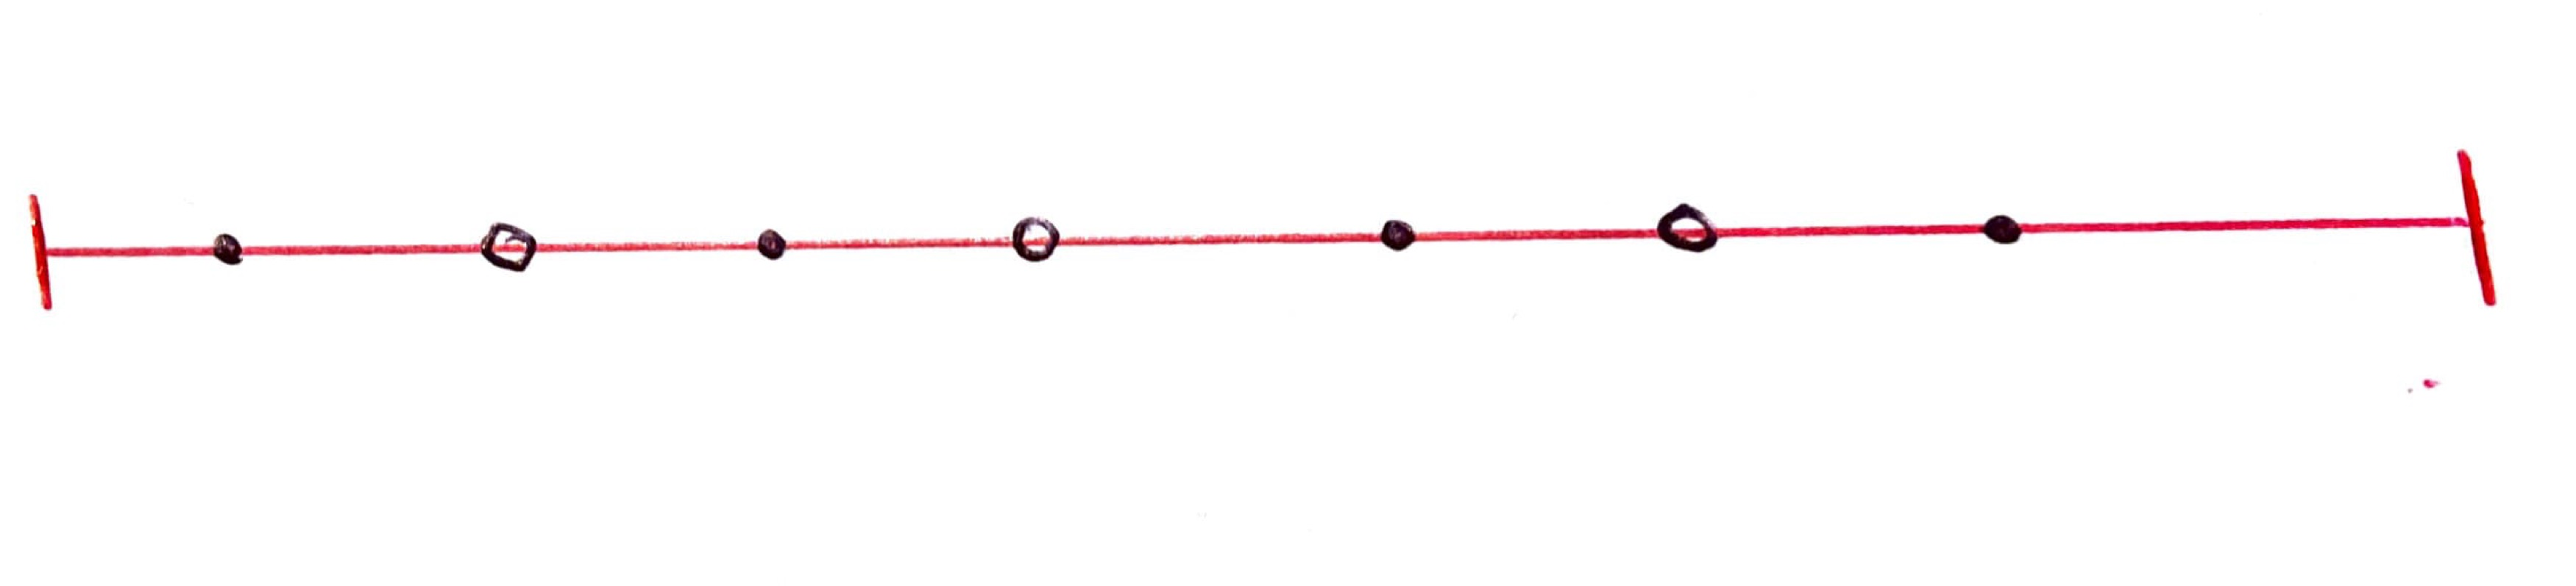
\includegraphics[width=0.7\linewidth]{red-black1}
		\caption{$1D$ grid (red (o) and black ($\cdot$) points }
		\label{fig:red-black1}
	\end{figure}
	
	
	\begin{figure}[H]
		\begin{subfigure}[b]{0.5\textwidth}
			\centering
			\includegraphics[width=1.0\linewidth]{"red-black"}
			\caption{}
			\label{fig:redblackgrid}
		\end{subfigure}
		%
		\begin{subfigure}[b]{0.5\textwidth}
			\centering
			\includegraphics[width=1.0\linewidth]{"stencil"}
			\caption{}
			\label{fig:redblackstencil}
		\end{subfigure}
		\caption{(a) and (b) respectively show $2D$ grid   and stencil for red-black with red (o) and black ($\cdot$) points }
	\end{figure}
	
	\subsection{Fourier Analysis (FA) to the two-grid operator.}
	
	FA has used to chose individual multigrid components for different situations, and it has also been applied in the calculation of convergence rates of MG methods while solving elliptic PDEs by using the exact eigenfunction of the discrete operator that is compatible with the boundary conditions \cite{kuo1989two}.\\
	
	\noindent  The corresponding Fourier representation  based on small subspaces of Fourier components for the relaxation method is possible to be calculated. Which means that the discrete fine-grid solution $u_{h}$  can be given by the linear combination of of Fourier components  that generate the whole space of bounded infinite grid functions.
	
	\noindent The error before and after the $i^{th}$ 2-grid-cycle is given by equations \eqref{f0} and \eqref{f00} respectively.
	
	\begin{equation}
		e_{h}^{(i)} = u_{h}^{(i-1)}  - u_{h} 
		\label{f0}
	\end{equation}

	\begin{equation}
	e_{h}^{(i)} = u_{h}^{(i)}  - u_{h} 
	\label{f00}
\end{equation}
	
	\noindent So their corresponding two-grid cycle error transformation is given by equation \eqref{f1};
	
	\begin{equation}
		e_{h}^{(i)} = M_{h}^{2h}e_{h}^{(i-1)}
		\label{f1}
	\end{equation}

	\noindent  with $M_{h}^{2h}$ is the error-transformation operator given by 
	\begin{equation}
	 M_{h}^{2h} = S_{h}^{\nu_{2}}K_{h}^{2h}S_{h}^{\nu_{1}} 
	\label{f2}
	\end{equation}
	
	 \noindent  where $K_{h}^{2h} = I_{h} - P_{2h}^{h}L_{2h}^{-1}R_{h}^{2h}L_{h}$ is the coarse-grid correction operator, $\nu_{1}$ and $\nu_{2}$ represent the number of pre- and postsmoothing iterations, $I_{h}$ the $G_{h}$ identity, $L_{2h}$ the approximation of $L_{h}$ on a coarse grid $G_{2h}$, $P_{2h}^{h}$ and $R_{2h}^{h}$ are transfer operators from coarse to fine grids and vice versa.\\
	 
	 \noindent In the 2D case, the Fourier space is divided into 4D spaces which introduces us to the spaces of $2h$-harmonics($\mathcal{F}_{2h}(\theta)$) that reads
	 
	 $$\mathcal{F}_{2h}(\theta) := span \{ \varphi _{h}(\mathbf{\theta}^{00},.), \varphi _{h}(\mathbf{\theta}^{10},.), \varphi _{h}(\mathbf{\theta}^{01},.)\}$$
	 
	 with $\mathbf{\theta} = \mathbf{\theta}^{00} \in \Theta_{2h} := (-\frac{\pi}{2},\frac{\pi}{2}]^{2},~ \mathbf{\theta^{\alpha} }:= \mathbf{\theta}^{00} - (\alpha_{1}\text{sign}(\theta_{1}), \alpha_{2}\text{sign}(\theta_{2}))\pi.$
	 
	 \noindent The standard coarsening $(H = 2h)$ is related $2h$-harmonics in the following mannar: $\Theta_{2h} = \Theta_{low},$ where low is taken as standard coarsening. Each low fequency 
	 $\mathbf{\theta}^{00} \in \Theta_{2h} $ is coupled with high frequencies $\theta^{\alpha} $ with $\alpha \ne (00)$ during the transistion from $G_{h}$ to $G_{2h}$.\\
	 
	\noindent On the coarse grid, the three high frequency components are not visible when coinciding with the corresponding low-frequency componet as given in equation \eqref{hf}.
	
	 \begin{equation}
	 	\varphi _{h}(\mathbf{\theta}^{00},x) = \varphi _{h}(\mathbf{\theta}^{11},x) = \varphi _{h}(\mathbf{\theta}^{10},x) = \varphi _{h}(\mathbf{\theta}^{01},x) \quad \text{for} \quad x \in G_{2h}
	 	\label{hf}
	 \end{equation}
	 
	\noindent Applying the periodicity of the exponential function, equation \eqref{hf}, can be verified by taking the Fourier components as coarse-grid functions as described in equation
	 \eqref{hf1}
	  \begin{equation}
	 	\varphi _{h}(\mathbf{\theta}^{00},x) = \varphi _{2h}(\mathbf{2\theta}^{00},x) = \varphi _{2h}(\mathbf{2\theta}^{\alpha},x) \text{with} \quad \mathbf{\theta}^{00} \in \Theta_{2h}, \,  x \in G_{2h}
	 	\label{hf1}
	 \end{equation}
\newpage	 
\noindent	Figure \ref{fig:FA}, represents a sample set of coupled frequencies. 
	
	 \begin{figure}[H]
	 	\centering
	 	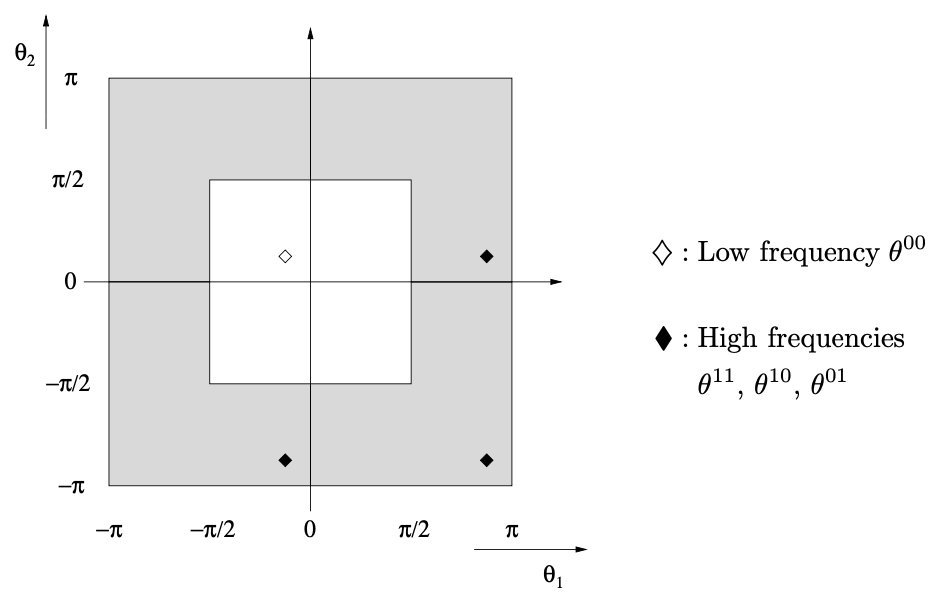
\includegraphics[width=0.7\linewidth]{FA}
	 	\caption{High and low Fourier frequencies generating a space of 2h- harmonics. Standard coarsening, d = 2. \cite{wienands2004practical} }
	 	\label{fig:FA}
	 \end{figure}
 
	 \noindent The coarse-grid correction ($K_{h}^{2h} = I_{h} -  P_{2h}^{h}L_{2h}^{-1} R_{h}^{2h} L_{h} $) leaves the $2h$-hamonics invariant space generating a simple ($4\times4$) block diagonal representation of $K_{h}^{2h}$ that reads
	 $$K_{h}^{2h}|_{\mathcal{F}_{2h}(\theta)} := K^{2g} (\theta) \quad (\theta \in \Theta_{2h}).$$
	 
	 \noindent The two grid method coarse grid correction with respect to the $2h$-hamonics invloves 
	 Fourier representation of the different operators depending on the prescribed order of  the multiindex $\alpha$. The Fourier smoothing analysis of the relaxation and coarse grid correction uses the order :
	 $$(0,0),~(1,1),~(1,0),~(0,1)$$
	 
	 \noindent  The Fourier components of  the fine grid discretization are eigen functions for a constant coefficient operators $L_{h} = [l_{k}]_{h}$. So the Foureir representation of  $L_{h}$ with respect to the $2h$-harmonics given by eqaution \eqref{fg}.
	 
	 \begin{equation}
	 	 L_{\mathcal{F}_{2h}(\theta)} = L^{2g}\theta =\begin{pmatrix}
	 	\tilde{L}_{h}(\mathbf{\theta}^{00})& 0 & 0 & 0 \\
	 		0 &\tilde{L}_{h}^{~}(\mathbf{\theta}^{11}) & 0 & 0 \\
	 		0 & 0 & \tilde{L}_{h}^{~}(\mathbf{\theta}^{10}) & 0 \\
	 		0 & 0 & 0 & \tilde{L}_{h}^{~}(\mathbf{\theta}^{01})
	 	\end{pmatrix} \in \mathbb{C}^{4\times4}
 	\label{fg}
	 \end{equation}
	 
	  \noindent where  $\tilde{L}_{h}(\mathbf{\theta}^{\alpha})$ are Fourier symbols given by $$\tilde{L}_{h}(\mathbf{\theta}^{\alpha}) = \sum_{\mathcal{K} \in J} l_{\mathcal{K}}\exp(i\mathcal{K} \theta^{\theta})$$
	
	 \noindent The coarse grid discretisation has two types of approximations: Discretization coarse grid approximation (DCA) and the Galerkin coarse grid approximation (GCA). This grid discretization $L_{2h}$ is given by:
	 $$L_{2h} = \tilde{R}_{h}^{2h} L_{h} \tilde{P}_{2h}^{h} $$
	 
	\noindent where $\tilde{R}_{h}^{2h}$ and $\tilde{P}_{2h}^{h}$ are the Galerkin transfer operators.
	\subsection{Discrete Sine Transform (DST)}
	This solver has been used in comparing and validating our results. it uses a signal at a discrete domain, and at the two ends of the arraydifferent variants corresponding to almost different odd/even boundary conditions.  Futhermore the solver expresses a function interms of a sinusoids with diffrernt frequencies and amplitudes implying different boundary conditions and an odd extension of the original signal \cite{gupta1990fast}.
	
	\subsection{Sparse Gaussian Elimination (SGE)}
	This solver uses sparse matrix (only a small fraction of the matrix elements are non zeros) capabilities to form D2x and D2y sparse matrices (see the appendix for more details). In this solver, pointers of some kind are explored to track the non zero entries, however costs are incured in storing and maniplating these pointers. Initially zero elements that don't fill-in are neither stored nor used as operands but  maximum advantage of these enntries is used by SGE in saving time and storage by not maniplating and storing these elements \cite{brayton1970some}.
	
	\subsection{Case Study}
	The above solvers are used to solve the following $2D$ Poison  problem \eqref{01}, and the solutions are displayed in the next section(Results).  The $2D$ elliptic problem is solved over the domain [a,b]x[a,b] with $a=0$ and $b=1$, grid spacing $dx=dy=h=\frac{b-a}{m+1}$, with $m=2^{k-1}$ where k =7 for this study. As a matter of fact, we used k = 7, since the method we are comparing with cant exceed that due to insufficient resources\ref{fig:spec}. But  Multigrid shoots more that, and the large the k the greater the accuracy.
	
	\begin{equation}
		\nabla ^{2} u = f(x,y)
		\label{01}
	\end{equation}
	where 
	$$f(x,y) = 10\pi^{2} (1+ \cos(4\pi(x+2y))) -2*\sin(2\pi(x+2y)) e^{sin(2\pi(x+2y))} $$
	with Boundary conditions.
	$$u(x,y) = g(x,y) $$
	where 
	$$g(x,y) = e^{sin(2\pi(x+2y))} $$
	
		\noindent The exact solution used to validate results and compute the error is given by equation \eqref{02}.
	
	\begin{equation}
		ue(x,y) = g(x,y)
		\label{02}
	\end{equation}
	
	\newpage
	\section{Results}
	Figure \ref{fig:jsoln} and \ref{fig:rdsoln} show the respective solutions obtained by using the two smothers: damped Gaus Jacobi and Red-black Gaus seidel.
	\begin{figure}[H]
		\begin{subfigure}[b]{0.5\textwidth}
			\centering
			\includegraphics[width=1.0\linewidth]{"uj"}
			\caption{}
			\label{fig:jsoln}
		\end{subfigure}
		%
		\begin{subfigure}[b]{0.5\textwidth}
			\centering
			\includegraphics[width=1.0\linewidth]{"ur"}
			\caption{}
			\label{fig:rdsoln}
		\end{subfigure}
		\caption{(a) and (b) respectively are solutions obtained using damped jacobi and Red-black smothers. }
	\end{figure}

		\noindent Figure \ref{fig:jerr} and \ref{fig:rderr} show the respective errors obtained by using the two smothers: damped Gaus Jacobi and Red-black Gaus seidel.
	
	\begin{figure}[h]
		\begin{subfigure}[b]{0.5\textwidth}
			\centering
			\includegraphics[width=1.0\linewidth]{"ej"}
			\caption{}
			\label{fig:jerr}
		\end{subfigure}
		%
		\begin{subfigure}[b]{0.5\textwidth}T
			\centering
			\includegraphics[width=1.0\linewidth]{"er"}
			\caption{}
			\label{fig:rderr}
		\end{subfigure}
		\caption{(a) and (b) respectively are errors obtained using damped jacobi and Red-black smothers. }
	\end{figure}
	
	\newpage
	\subsection{Comparison and Validation of Results}
	The obtained solution for MG is validated against the DST solver result as shown in figures \ref{fig:dstsoln} and \ref{fig:ujsoln}. According to  figures \ref{fig:edst} and \ref{fig:ej}, these error plots  depict that the results obatined are realistic, since both have an upper bound error of magnitude $10^{-3}$.\\ 
	
	\begin{figure}[H]
		\begin{subfigure}[b]{0.5\textwidth}
			\centering
			\includegraphics[width=1.0\linewidth]{"udst"}
			\caption{}
			\label{fig:dstsoln}
		\end{subfigure}
		%
		\begin{subfigure}[b]{0.5\textwidth}
			\centering
			\includegraphics[width=1.0\linewidth]{"uj"}
			\caption{}
			\label{fig:ujsoln}
		\end{subfigure}
		\caption{(a) and (b) respectively are solutions obtained using DST and Multigrid solver with damped Jacobi smother. }
	\end{figure}
	
	\begin{figure}[H]
		\begin{subfigure}[b]{0.5\textwidth}
			\centering
			\includegraphics[width=1.0\linewidth]{"edst"}
			\caption{}
			\label{fig:edst}
		\end{subfigure}
		%
		\begin{subfigure}[b]{0.5\textwidth}
			\centering
			\includegraphics[width=1.0\linewidth]{"ej"}
			\caption{}
			\label{fig:ej}
		\end{subfigure}
		\caption{(a) and (b) respectively are errors obtained using DST and Multigrid solver with damped Jacobi smother. }
	\end{figure}

\noindent A computational time cost check was performed, as a comparision with SGE, DST, and MG solvers on three different runs for $k = 4,5,6,7$ , and results are depicted in table \ref{fig:walltime}. The results displayed in table \ref{fig:walltime}, look to be random, but the trend shows that run time decreases as h increases for DST, but for MG and SGE, appears to be the reverse. Thats why we hard to take the mean time to obtain the best minimum wall time for each run as displayed in table \ref{fig:meant}.

\begin{figure}[H]
	\centering
	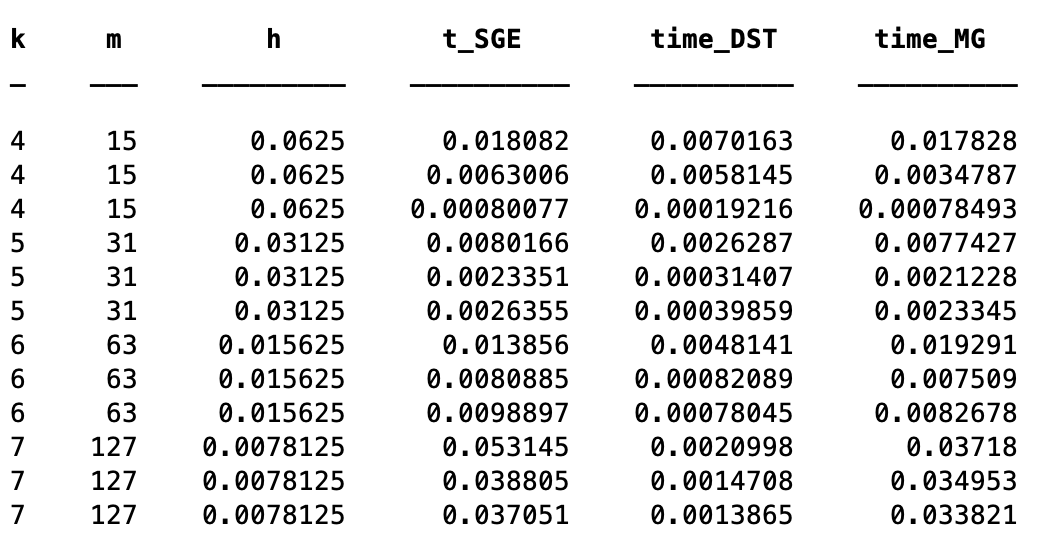
\includegraphics[width=0.7\linewidth]{walltime}
	\caption{Wall time at each run}
	\label{fig:walltime}
\end{figure}

\noindent According to the computed mean wall clock time shown in Table \ref{fig:meant}, DST
appears to be the best since it has the lowest computation time  amongest all other method as m increases followed by MG (using damped Jacobi smoother). However SGE also compited with MG due to the use of the sparse matrix that quickens the computations.
\begin{figure}[H]
	\centering
	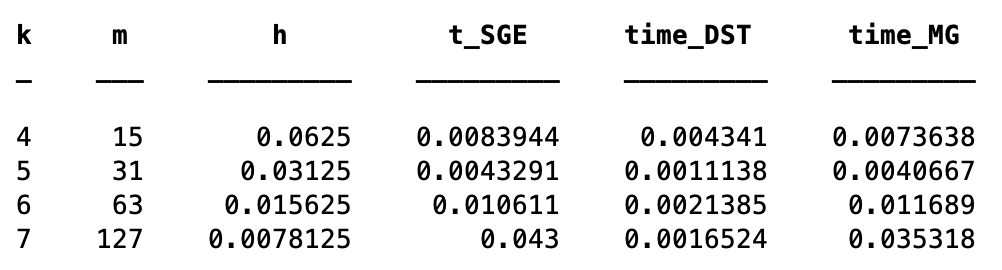
\includegraphics[width=0.7\linewidth]{meant}
	\caption{Mean wall time }
	\label{fig:meant}
\end{figure}
\noindent \textbf{Note:} I used only $k$ values from $4$ to $5$, because when i tried to run for $k = 8$ and above  the MATLAB on my computer terminated for SGE, so i wouldnot perform any further simulations beyond $k=7$.  But for MG and DST i was able to do simulations for $k\ge7$.

\noindent The simulations were perfomed on a computer with these the following specifications as shown in figure \ref{fig:spec}. Its concluded that simulations depend much on different systems specifications. 

\begin{figure}[H]
	\centering
	\includegraphics[width=0.5\linewidth]{"Screenshot 2021-03-19 at 12.49.12 PM"}
	\caption{Computer specifications}
	\label{fig:spec}
\end{figure}
	
	\section{Conclusion}
	This section discusses about the conclusions deduced from the above methods used. All the objectives have been well implemeted and achived.\\
	
		\noindent We used the Discrete Sine Transform (DST) to compare and validate our solution. And according to figures \ref{fig:dstsoln}, \ref{fig:ujsoln}, \ref{fig:edst}, and \ref{fig:ej}, we were able to validate our solution since the results dipict the same solution and magnitude of the error ($10^{-3}$). However using bigger $k$ values we obtain better results and better error tolerance much smaller than  ($10^{-3}$). But we were restricted to use $k\ge 8$ since SGE couldn't perform for $k\ge 8$, so for a fair comparison i had to use $k < 8$.  \\
	
	\noindent According to table \ref{fig:meant}, overall, DST wins in terms of cost, however the mean wall time for MG, is similar to the two methods we are validating with, hence the results obtained from using MG to solve the same problem are realistic.\\
	
	\noindent In a case where the matrix of the original equation is symmetric positive definite (SPD), then a multgrid method with a forced reduced tolerance may be used as a preconditioner, however, the SPD constraint makes construction of the preconditioner complicated.

	\bibliographystyle{plain}
	\bibliography{document}
	
	\section{Appendix}
	
	
	\subsection{MG solver}
	\begingroup\makeatletter\def\@currenvir{verbatim}
	\verbatim
	% ===============================================================================
	% Author      : Prof. Grady wright 
	% modified by : Brian Kyanjo
	% Class       : MATH566
	% Date        : March 18th, 2021
	%
	% Numerical approximation to Poisson's equation over the square [a,b]x[a,b] with
	% Dirichlet boundary conditions.  Uses a uniform mesh with (n+2)x(n+2) total
	% points (i.e, n interior grid points). 
	%
	% Solves with classical multigrid (v-cycle and damped-Jacobi, and red-black Gaus 
	% Seidel smoother).
	%
	% Input:
	%     ffun : the RHS of poisson equation (i.e. the Laplacian of u).
	%     gfun : the boundary function representing the Dirichlet B.C.
	%      a,b : the interval defining the square
	%        m : m+2 is the number of points in either direction of the mesh.
	% smoother : Selection of the smoother.
	% Ouput:
	%        u : the numerical solution of Poisson equation at the mesh points.
	%      x,y : the uniform mesh.
	%
	% ===============================================================================
	function [u,x,y] = multigrid_solver(ffun,gfun,a,b,m)
	
	k = round(log2(m+1));
	
	if abs(log2(m+1)-k) > 100*eps
	error('multigrid_solver:power2','m+1 must be a power of 2');
	end
	
	h = (b-a)/2^k;   % Mesh spacing
	
	[x,y] = meshgrid(a:h:b);   % Uniform mesh, including boundary points.
	
	idx = 2:m+1;
	idy = 2:m+1;
	
	% Compute boundary terms, south, north, east, west
	ubs = feval(gfun,x(1,1:m+2),y(1,1:m+2));     % Include corners
	ubn = feval(gfun,x(m+2,1:m+2),y(m+2,1:m+2)); % Include corners
	ube = feval(gfun,x(idy,m+2),y(idy,m+2));     % No corners
	ubw = feval(gfun,x(idy,1),y(idy,1));         % No corners
	
	% Evaluate the RHS of Poisson's equation at the interior points.
	f = feval(ffun,x,y);
	
	% Inital guess
	u = zeros(m+2,m+2);
	
	% Add boundary terms to u
	u(idx,1) = ubw; u(idx,m+2) = ube;
	u(1,:) = ubs; u(m+2,:) = ubn;
	
	tol = 1e-8;
	r = inf;
	nrmf = norm(f(:));
	while norm(r(:)) > tol*nrmf
	[u,r] = vcycle(u,f,h,k);
	end
	
	end
	
	function [u,r] = vcycle(u,f,h,k)
	
	numSmooths = 3;
	n = 2^k; n2 = n/2;
	i = 2:n; i2 = 2:n2;
	
	if k == 1
	% Only one interior point so solve the system:
	u(2,2) = 0.25*(u(1,2)+u(3,2)+u(2,1)+u(2,3)-h^2*f(2,2));
	return;
	else
	% Smooth the solution.
	%Choice of the smoother
	smoother = 2;  %1 for Damped Jacobi smoother 
	%2 for red-black-Gaus smoother
	
	if smoother == 1
	u = dampedJacobi(u,f,h,k,numSmooths);
	elseif  smoother == 2
	u = redblack(u,f,h,k,numSmooths);
	end
	
	% Calculate residual
	r = zeros(n+1);
	r(i,i) = f(i,i) - (-4*u(i,i)+u(i-1,i)+u(i+1,i)+u(i,i-1)+u(i,i+1))/h^2;
	
	% Restrict the residual to the coarser grid using full-weighting
	jj = 3:2:n-1;
	f2 = zeros(n2+1);
	f2(i2,i2) = (r(jj-1,jj)+r(jj+1,jj)+r(jj,jj-1)+r(jj,jj+1)+4*r(jj,jj))/8;
	
	% Repeat call to vcylce with the residual on coarser grid and with a
	% zero initial guess.
	u2 = vcycle(zeros(n2+1),f2,2*h,k-1);
	
	% Interpolate (prolongate) the correction to the finer grid
	ut = zeros(n+1);
	ut(1:2:n+1,1:2:n+1) = u2;
	ut(2:2:n,1:2:n+1) = 0.5*(u2(1:n2,:)+u2(2:n2+1,:));
	ut(:,2:2:n+1) = 0.5*(ut(:,1:2:n-1)+ut(:,3:2:n+1));
	
	% Update the solution and smooth again:    
	if smoother == 1
	u = dampedJacobi(u+ut,f,h,k,numSmooths);
	elseif  smoother == 2
	u = redblack(u+ut,f,h,k,numSmooths);
	end
	
	% Calculate residual
	r(i,i) = f(i,i) - (-4*u(i,i)+u(i-1,i)+u(i+1,i)+u(i,i-1)+u(i,i+1))/h^2;
	end
	end
	
	%Damped Jacobi smoother
	function u = dampedJacobi(u,f,h,k,numSmooths)
	omega = 4/5;
	n = 2^k;
	i = 2:n;
	f = h^2*f;
	% Smooth u using underrelaxed Jacobi
	for j=1:numSmooths
	u(i,i) = (0.25*omega)*(u(i-1,i)+u(i+1,i)+u(i,i-1)+u(i,i+1)-f(i,i)) + ...
	(1-omega)*u(i,i);
	end
	
	end
	
	%Red black Gauss-Seidel step
	function u = redblack(u,f,h,k,numSmooths)
	n = 2^k;
	f = h^2*f;
	for k = 1:numSmooths
	%Red points
	for i = 2:n
	for j = 2:n
	if (mod(i+j,2) == 0) %sum of indices is even
	u(i,j) = 0.25*(u(i-1,j)+u(i+1,j)...
	+u(i,j-1)+u(i,j+1) - f(i,j));
	end
	end
	end
	
	%Black points
	for i = 2:n
	for j = 2:n
	if (mod(i+j,2) == 1) %sum of indices is odd
	u(i,j) = 0.25*(u(i-1,j)+u(i+1,j)...
	+u(i,j-1)+u(i,j+1) - f(i,j));
	end
	end
	end
	end
	end
\end{verbatim}

\subsection{DST Solver}
\begingroup\makeatletter\def\@currenvir{verbatim}
\verbatim

% ===============================================================================
% Author      : Prof. Grady wright 
% modified by : Brian Kyanjo
% Class       : MATH566
% Date        : March 18th, 2021
%
% Numerical approximation to Poisson's equation over the square [a,b]x[a,b] with
% Dirichlet boundary conditions.  Uses a uniform mesh with (n+2)x(n+2) total
% points (i.e, n interior grid points). 
%
% Solves with the DST.
%
% Input:
%     pfun : the RHS of poisson equation (i.e. the Laplacian of u).
%     bfun : the boundary function representing the Dirichlet B.C.
%      a,b : the interval defining the square
%        m : m+2 is the number of points in either direction of the mesh.
% Ouput:
%        u : the numerical solution of Poisson equation at the mesh points.
%      x,y : the uniform mesh.
% ===============================================================================

function [u,x,y] = dst_solver(pfun,bfun,a,b,m)

h = (b-a)/(m+1);   % Mesh spacing

[x,y] = meshgrid(a:h:b);   % Uniform mesh, including boundary points.

idx = 2:m+1;
idy = 2:m+1;

% Compute boundary terms, south, north, east, west
ubs = feval(bfun,x(1,1:m+2),y(1,1:m+2));     % Include corners
ubn = feval(bfun,x(m+2,1:m+2),y(m+2,1:m+2)); % Include corners
ube = feval(bfun,x(idy,m+2),y(idy,m+2));     % No corners
ubw = feval(bfun,x(idy,1),y(idy,1));         % No corners

% Evaluate the RHS of Poisson's equation at the interior points.
f = feval(pfun,x(idy,idx),y(idy,idx));

% Adjust f for boundary terms
f(:,1) = f(:,1) - ubw/h^2;             % West
f(:,m) = f(:,m) - ube/h^2;             % East
f(1,1:m) = f(1,1:m) - ubs(idx)/h^2;    % South
f(m,1:m) = f(m,1:m) - ubn(idx)/h^2;    % North

% Computation of fhat=(S*f)*S^(-1), where S is the discrete sine transform.
fhat = idst(dst(f,1),2);

% Denominator for the computation of uhat:
denom = bsxfun(@plus,cos(pi*(idx-1)./(m+1)).',cos(pi*(idx-1)./(m+1)))-2;

uhat = h^2/2*(fhat./denom);

% Computation of u = (S^(-1)*uhat)*S
u = dst(idst(uhat,1),2);

% Append on to u the boundary values from the Dirichlet condition.
u = [ubs;[ubw,u,ube];ubn];

end

\end{verbatim}

	\subsection{SGE Solver}
	\begingroup\makeatletter\def\@currenvir{verbatim}
	\verbatim

% ===============================================================================
% Author      : Prof. Grady wright 
% modified by : Brian Kyanjo
% Class       : MATH566
% Date        : March 18th, 2021
%
% Numerical approximation to Poisson's equation over the square [a,b]x[a,b] with
% Dirichlet boundary conditions.  Uses a uniform mesh with (n+2)x(n+2) total
% points (i.e, n interior grid points).
% Input:
%     ffun : the RHS of poisson equation (i.e. the Laplacian of u).
%     gfun : the boundary function representing the Dirichlet B.C.
%      a,b : the interval defining the square
%        m : m+2 is the number of points in either direction of the mesh.
% Ouput:
%        u : the numerical solution of Poisson equation at the mesh points.
%      x,y : the uniform mesh.
% ===============================================================================

function [u,x,y] = sge_solver(ffun,gfun,a,b,m)

h = (b-a)/(m+1);   % Mesh spacing

[x,y] = meshgrid(a:h:b);   % Uniform mesh, including boundary points.

idx = 2:m+1;
idy = 2:m+1;

% Compute boundary terms, south, north, east, west
ubs = feval(gfun,x(1,1:m+2),y(1,1:m+2));     % Include corners
ubn = feval(gfun,x(m+2,1:m+2),y(m+2,1:m+2)); % Include corners
ube = feval(gfun,x(idy,m+2),y(idy,m+2));     % No corners
ubw = feval(gfun,x(idy,1),y(idy,1));         % No corners

% Evaluate the RHS of Poisson's equation at the interior points.
f = feval(ffun,x(idy,idx),y(idy,idx));

% Adjust f for boundary terms
f(:,1) = f(:,1) - ubw/h^2;             % West
f(:,m) = f(:,m) - ube/h^2;             % East
f(1,1:m) = f(1,1:m) - ubs(idx)/h^2;    % South
f(m,1:m) = f(m,1:m) - ubn(idx)/h^2;    % North

f = reshape(f,m*m,1);

%Using sparse matrix capabilities to form D2x and D2y matrices
I = eye(m);
e = ones(m,1);
e1 = zeros(m,1);

%D2x
T = spdiags([e1 -2*e1 e1],[-1 0 1],m,m);
S = spdiags([e e],[-1 1],m,m);
D2x = (1/h^2)*(kron(I, T) + kron(S,I));

%D2y
Ty = spdiags([e -2*e e],[-1 0 1],m,m);
Sy = spdiags([e1 e1],[-1 1],m,m);
D2y = (1/h^2)*(kron(I, Ty) + kron(Sy,I));

% Solve the system
u = (D2x + D2y)\f;

% Convert u from a column vector to a matrix to make it easier to work with
% for plotting.
u = reshape(u,m,m);

% Append on to u the boundary values from the Dirichlet condition.
u = [ubs;[ubw,u,ube];ubn];

end


\end{verbatim}
	
	\subsection{Main}
	\begingroup\makeatletter\def\@currenvir{verbatim}
	\verbatim
	
	%==========================================================================
	% Author        : Brian Kyanjo
	% Supervised by : Prof. Grady wright 
	% Class         : MATH566
	% Date          : March 18th, 2021
	%
	% Main code for calling all necessary functions. And the sample fuctions to
	% be used are defined here.
	% Multigrid and DST solvers are used to solve the problem in question.
	% The wall time and mean wall time for each method in 3 runs has been
	% performed.
	%==========================================================================
	
	clear all;
	close all;
	
	% Script for testing fd2poisson over the square [a,b]x[a,b]
	a = 0; b = 1;
	
	% Laplacian(u) = f
	f = @(x,y) 10*pi^2*(1+cos(4*pi*(x+2*y))-2*sin(2*pi*(x+2*y))).*exp(sin(2*pi*(x+2*y)));  
	% u = g on Boundary
	g = @(x,y) exp(sin(2*pi*(x+2*y)));            
	
	%Exact solution is g.
	uexact = @(x,y) g(x,y);
	
	% Compute and time the solution
	k1 = zeros(1,4); h1 = zeros(1,4); m1 = zeros(1,4); 
	t = zeros(1,4); 
	t_dst = zeros(1,4); 
	t_mg = zeros(1,4);
	
	t1 = [];
	tdst = [];
	tmg = [];
	for ii=1:3
	for k=4:7
	%k=10;
	
	k1(k-3) = k;
	m1(k-3) = 2^k-1;
	m = 2^k-1; 
	h1(k-3) = (b-a)/(m+1);
	h = (b-a)/(m+1);
	
	tic
	[u,x,y] = sge_solver(f,g,a,b,m);
	gedirect = toc;
	t(k-3) = gedirect;
	
	tic
	[udst,x,y] = dst_solver(f,g,a,b,m);
	gedirect = toc;
	t_dst(k-3) = gedirect;
	
	tic
	[umg,x,y] = multigrid_solver(f,g,a,b,m);
	gedirect = toc;
	t_mg(k-3) = gedirect;
	end 
	t1 = [t1,t];
	tdst = [tdst, t_dst]; 
	tmg = [tmg,t_mg];
	end
	
	%k=4
	c4=[t1(1);t1(5);t1(9)]'; 
	fd4=[tdst(1);tdst(5);tdst(9)]'; 
	h4=[tmg(1);tmg(5);tmg(9)]';
	
	%k=5
	c5=[t1(2);t1(6);t1(10)]'; 
	fd5=[tdst(2);tdst(6);tdst(10)]'; 
	h5=[tmg(2);tmg(6);tmg(10)]';
	
	%k=6
	c6=[t1(3);t1(7);t1(11)]'; 
	fd6=[tdst(3);tdst(7);tdst(11)]'; 
	h6=[tmg(3);tmg(7);tmg(11)]';
	
	%k=7
	c7=[t1(4);t1(8);t1(12)]'; 
	fd7=[tdst(4);tdst(8);tdst(12)]'; 
	h7=[tmg(4);tmg(8);tmg(12)]';
	
	k4 = [k1(1);k1(1);k1(1)];
	m4 = [m1(1);m1(1);m1(1)];
	h_4 = [h1(1);h1(1);h1(1)];
	
	%Table showing timing results of each method and for each value of m.
	Table4 = table(k4,m4,h_4,c4(:),fd4(:),h4(:), 'VariableNames',{'k','m','h','t_SGE','time_DST','time_MG'});
	
	k5 = [k1(2);k1(2);k1(2)];
	m5 = [m1(2);m1(2);m1(2)];
	h_5 = [h1(2);h1(2);h1(2)];
	%Table showing timing results of each method and for each value of m.
	Table5 = table(k5,m5,h_5,c5(:),fd5(:),h5(:), 'VariableNames',{'k','m','h','t_SGE','time_DST','time_MG'});
	
	k6 = [k1(3);k1(3);k1(3)];
	m6 = [m1(3);m1(3);m1(3)];
	h_6 = [h1(3);h1(3);h1(3)];
	%Table showing timing results of each method and for each value of m.
	Table6 = table(k6,m6,h_6,c6(:),fd6(:),h6(:), 'VariableNames',{'k','m','h','t_SGE','time_DST','time_MG'});
	
	k7 = [k1(4);k1(4);k1(4)];
	m7 = [m1(4);m1(4);m1(4)];
	h_7 = [h1(4);h1(4);h1(4)];
	%Table showing timing results of each method and for each value of m.
	Table7 = table(k7,m7,h_7,c7(:),fd7(:),h7(:), 'VariableNames',{'k','m','h','t_SGE','time_DST','time_MG'});
	
	
	%General Table
	Table = [Table4; Table5; Table6; Table7]
	
	
	%mean
	Tablem4 = table(k1(1),m1(1),h1(1),mean(c4),mean(fd4),mean(h4), 'VariableNames',{'k','m','h','t_SGE','time_DST','time_MG'});
	Tablem5 = table(k1(2),m1(2),h1(2),mean(c5),mean(fd5),mean(h5), 'VariableNames',{'k','m','h','t_SGE','time_DST','time_MG'});
	Tablem6 = table(k1(3),m1(3),h1(3),mean(c6),mean(fd6),mean(h6), 'VariableNames',{'k','m','h','t_SGE','time_DST','time_MG'});
	Tablem7 = table(k1(4),m1(4),h1(4),mean(c7),mean(fd7),mean(h7), 'VariableNames',{'k','m','h','t_SGE','time_DST','time_MG'});
	
	Table_mean = [Tablem4; Tablem5; Tablem6; Tablem7]
	
	% 
	% % Plot solution
	% figure, set(gcf,'DefaultAxesFontSize',10,'PaperPosition', [0 0 3.5 3.5]), 
	% surf(x,y,udst), xlabel('x'), ylabel('y'), zlabel('u(x,y)'),
	% title(strcat('Numerical Solution,udst, to Poisson Equation, h=',num2str(h)));
	% 
	% % Plot error
	% figure, set(gcf,'DefaultAxesFontSize',10,'PaperPosition', [0 0 3.5 3.5]), 
	% surf(x,y,udst-uexact(x,y)),xlabel('x'),ylabel('y'), zlabel('Error'), 
	% title(strcat('Errordst, h=',num2str(h)));
	
	
	% %Plot solution
	% figure, set(gcf,'DefaultAxesFontSize',10,'PaperPosition', [0 0 3.5 3.5]), 
	% surf(x,y,umg), xlabel('x'), ylabel('y'), zlabel('u(x,y)'),
	% title(strcat('Numerical Solution,umg, to Poisson Equation, h=',num2str(h)));
	% 
	% %Plot error
	% figure, set(gcf,'DefaultAxesFontSize',10,'PaperPosition', [0 0 3.5 3.5]), 
	% surf(x,y,umg-uexact(x,y)),xlabel('x'),ylabel('y'), zlabel('Error'), 
	% title(strcat('Errormg, h=',num2str(h)));
	
\end{verbatim}

\end{document}